% **************************************************
% Document Class Definition
% **************************************************
\documentclass[%
    paper=A4,               % paper size --> A4 is default in Germany
    twoside=true,           % onesite or twoside printing
    openright,              % doublepage cleaning ends up right side
    parskip=half,           % spacing value / method for paragraphs
    chapterprefix=true,     % prefix for chapter marks
    11pt,                   % font size
    headings=normal,        % size of headings
    bibliography=totoc,     % include bib in toc
    listof=totoc,           % include listof entries in toc
    titlepage=on,           % own page for each title page
    captions=tableabove,    % display table captions above the float env
    chapterprefix=false,    % do not display a prefix for chapters
    appendixprefix=false,    % but display a prefix for appendix chapter
    draft=false,            % value for draft version
]{scrreprt}%


% **************************************************
% Setup YOUR thesis document in this file !
% **************************************************
% !TEX root = my-thesis.tex


% **************************************************
% Files' Character Encoding
% **************************************************
\PassOptionsToPackage{utf8}{inputenc}
\usepackage{inputenc}


% **************************************************
% Information and Commands for Reuse
% **************************************************
\newcommand{\thesisTitle}{Applying Machine Learning Techniques to Simulated and Experimental Data from the Wendelstein 7-X}
\newcommand{\thesisName}{Nathan Belmore}
\newcommand{\thesisSubject}{M.Sc. Physik}
\newcommand{\thesisDate}{Dec 10th, 2022}
\newcommand{\thesisVersion}{Revision 3}

\newcommand{\thesisFirstReviewer}{Prof. Thomas Sunn Pedersen}
\newcommand{\thesisFirstReviewerUniversity}{\protect{Universität Greifswald}}
\newcommand{\thesisFirstReviewerDepartment}{Department of Physics}

\newcommand{\thesisSecondReviewer}{Prof. Ralf Schneider}
\newcommand{\thesisSecondReviewerUniversity}{\protect{Universität Greifswald}}
\newcommand{\thesisSecondReviewerDepartment}{Department of Physics}

\newcommand{\thesisFirstSupervisor}{Daniel Böckenhoff}
\newcommand{\thesisSecondSupervisor}{John Smith}

\newcommand{\thesisUniversity}{\protect{Universität Greifswald}}
\newcommand{\thesisUniversityDepartment}{Department of Physics}
\newcommand{\thesisUniversityInstitute}{with support from the Max-Planck Institute for Plasma Physics}
\newcommand{\thesisUniversityCity}{Greifswald}
\newcommand{\thesisUniversityStreetAddress}{Felix-Hausdorff-Straße 6, Germany}
\newcommand{\thesisUniversityPostalCode}{17489}


% **************************************************
% Debug LaTeX Information
% **************************************************
%\listfiles


% **************************************************
% Load and Configure Packages
% **************************************************
\usepackage[english]{babel} % babel system, adjust the language of the content
\PassOptionsToPackage{% setup clean thesis style
    figuresep=colon,%
    hangfigurecaption=false,%
    hangsection=true,%
    hangsubsection=true,%
    sansserif=false,%
    configurelistings=true,%
    colorize=full,%
    colortheme=bluemagenta,%
    configurebiblatex=true,%
    bibsys=biber,%
    bibfile=bib-refs,%
    bibstyle=numeric,%
    bibsorting=nty,%
}{cleanthesis}
\usepackage{cleanthesis}

\hypersetup{% setup the hyperref-package options
    pdftitle={\thesisTitle},    %   - title (PDF meta)
    pdfsubject={\thesisSubject},%   - subject (PDF meta)
    pdfauthor={\thesisName},    %   - author (PDF meta)
    plainpages=false,           %   -
    colorlinks=false,           %   - colorize links?
    pdfborder={0 0 0},          %   -
    breaklinks=true,            %   - allow line break inside links
    bookmarksnumbered=true,     %
    bookmarksopen=true          %
}

% **************************************************
% Other Packages
% **************************************************
\usepackage{scrhack}
\usepackage{multirow}
\usepackage{amsmath}
\usepackage{tikz}
\setlength{\arrayrulewidth}{0.5mm}
\setlength{\tabcolsep}{18pt}
\renewcommand{\arraystretch}{1.5}


% **************************************************
% Document CONTENT
% **************************************************
\begin{document}

% uncomment the following command to fill up pages with
% whitespace instead of aligning the first and last lines
% of a page (see \raggedbottom vs. \flushbottom)
%\raggedbottom

% --------------------------
% rename document parts
% --------------------------

% > set short label names for floating environments figure and table
%\renewcaptionname{ngerman}{\figurename}{Abb.}
%\renewcaptionname{ngerman}{\tablename}{Tab.}
\renewcaptionname{english}{\figurename}{Fig.}
\renewcaptionname{english}{\tablename}{Tab.}

% > rename the title of the LOL, i.e. list of listings (default is "Listings")
\renewcommand*{\lstlistlistingname}{List of Listings}

% --------------------------
% Front matter
% --------------------------
\pagenumbering{roman}			% roman page numbing (invisible for empty page style)
\pagestyle{empty}				% no header or footers
% !TEX root = ../my-thesis.tex
%
% ------------------------------------  --> cover title page
\begin{titlepage}
	\pdfbookmark[0]{Cover}{Cover}
	\flushright
	\hfill
	\vfill
	{\LARGE\thesisTitle \par}
	\rule[5pt]{\textwidth}{.4pt} \par
	{\Large\thesisName}
	\vfill
	\textit{\large\thesisDate} \\
	Version: \thesisVersion
\end{titlepage}


% ------------------------------------  --> main title page
\begin{titlepage}
	\pdfbookmark[0]{Titlepage}{Titlepage}
	\tgherosfont
	\centering

	{\Large \thesisUniversity} \\[4mm]
	
\includegraphics[width=6cm]{images/unilogo} \\[2mm]
	\textsf{\thesisUniversityDepartment} \\
	\textsf{\thesisUniversityInstitute} \\
	% \textsf{\thesisUniversityGroup} \\

	\vfill
	{\large \thesisSubject} \\[5mm]
	{\LARGE \color{ctcolortitle}\textbf{\thesisTitle} \\[10mm]}
	{\Large \thesisName} \\

	\vfill
	\begin{minipage}[t]{.27\textwidth}
		\raggedleft
		\textit{1. Reviewer}
	\end{minipage}
	\hspace*{15pt}
	\begin{minipage}[t]{.65\textwidth}
		{\Large \thesisFirstReviewer} \\
		{\small \thesisFirstReviewerDepartment} \\[-1mm]
		{\small \thesisFirstReviewerUniversity}
	\end{minipage} \\[5mm]
	\begin{minipage}[t]{.27\textwidth}
		\raggedleft
		\textit{2. Reviewer}
	\end{minipage}
	\hspace*{15pt}
	\begin{minipage}[t]{.65\textwidth}
		{\Large \thesisSecondReviewer} \\
		{\small \thesisSecondReviewerDepartment} \\[-1mm]
		{\small \thesisSecondReviewerUniversity}
	\end{minipage} \\[10mm]
	\begin{minipage}[t]{.27\textwidth}
		\raggedleft
		\textit{Supervisors}
	\end{minipage}
	\hspace*{15pt}
	\begin{minipage}[t]{.65\textwidth}
		\thesisFirstSupervisor\
	\end{minipage} \\[10mm]

	\thesisDate \\

\end{titlepage}


% ------------------------------------  --> lower title back for single page layout
\hfill
\vfill
{
	\small
	\textbf{\thesisName} \\
	\textit{\thesisTitle} \\
	\thesisSubject, \thesisDate \\
	Reviewers: \thesisFirstReviewer\ and \thesisSecondReviewer \\
	Supervisors: \thesisFirstSupervisor\ \\[1.5em]
	\textbf{\thesisUniversity} \\
	% \textit{\thesisUniversityGroup} \\
	\thesisUniversityDepartment \\
	\thesisUniversityInstitute \\
	\thesisUniversityStreetAddress \\
	\thesisUniversityPostalCode\ and \thesisUniversityCity
}
		% INCLUDE: all titlepages
\cleardoublepage

\pagestyle{plain}				% display just page numbers
% !TEX root = ../my-thesis.tex
%
\pdfbookmark[0]{Abstract}{Abstract}
\addchap*{Abstract}
\label{sec:abstract}

The Wendelstein 7-X (W7-X) plasma experiment is the most advanced stellarator of the HELIAS type. W7-X aims to demonstrate the feasibility of steady-state operation of a plasma experiment and the potential viability of a fusion reactor. W7-X is a device with a five-fold symmetry and with a unique magnetic field geometry created using non-planar and planar superconducting coils. It also uses the island divertor concept for managing heat and particle exhaust at the plasma-wall interfaces, which are created by divertor target plates intersecting the edge magnetic islands. The graphite divertor targets used in W7-X are designed to withstand a heat load of up to 10 $MW/m^2$, but exceeding this limit can damage the divertor structures and prevent sustained operation of the device. In order to prevent thermal overload, the positions of the edge magnetic islands with respect to the target plates can be adjusted using trim and control coils. This thesis presents an approach for inferring the edge rotational transform, a key parameter that determines the position of the magnetic islands and heat load pattern, from infrared camera data. Using an inceptnet convolutional neural network, the 520x130 input resolution is a good compromise between computational cost and network performance. When evaluating $\iota$, the rotational transform, this network is able to achieve an $rmse$ of $4.13 \cdot 10^{-3}$ and a training time of less than a day on a single GPU, which is an order of magnitude better than prior work with similar data.		% INCLUDE: the abstracts (english and german)
\cleardoublepage
% %
% % !TEX root = ../my-thesis.tex
%
\pdfbookmark[0]{Acknowledgement}{Acknowledgement}
\addchap*{Acknowledgement}
\label{sec:acknowledgement}

\Blindtext[2][2]
 % INCLUDE: acknowledgement
\cleardoublepage
%
\currentpdfbookmark{\contentsname}{toc}
\setcounter{tocdepth}{2}		% define depth of toc
\tableofcontents				% display table of contents
\cleardoublepage

% --------------------------
% Body matter
% --------------------------
\pagenumbering{arabic}			% arabic page numbering
\setcounter{page}{1}			% set page counter
\pagestyle{scrheadings}			% header and footer style

%% Uncomment the following lines using the \part command
%% to add part sections
%\part{Example Part}
% !TEX root = ../my-thesis.tex
%
\chapter{Introduction}
\label{sec:intro}

\cleanchapterquote{You can’t do better design with a computer, but you can speed up your work enormously.}{Wim Crouwel}{(Graphic designer and typographer)}

Machine learning has launched a new era of real time datat analysis and control.
As a result, it is now possible to do real time analysis and control that was unthinkable in the past.
Problems where machine learning can really be taken advantage of are problems whose solutions are too complex for traditional algorithmic approaches on the timescale of the events.

In the world of nuclear fusion we find many problems like this. Nuclear fusion is a complex atomic, theromodynamic, and electromagnetic problem.
To achieve fusion it is neccery to overcome the nuclei's postive charge.

\section{Postcards: My Address}
\label{sec:intro:address}

\textbf{Ricardo Langner} \\
Alfred-Schrapel-Str. 7 \\
01307 Dresden \\
Germany



\section{Motivation and Problem Statement}
\label{sec:intro:motivation}

\Blindtext[3][1] \cite{Jurgens:2000,Jurgens:1995,Miede:2011,Kohm:2011,Apple:keynote:2010,Apple:numbers:2010,Apple:pages:2010}

\section{Results}
\label{sec:intro:results}

\Blindtext[1][2]

\subsection{Some References}
\label{sec:intro:results:refs}

\cite{WEB:GNU:GPL:2010,WEB:Miede:2011}
\Blindtext[1][1]

\subsubsection{Methodology}
\label{sec:intro:results:refs:method}

\Blindtext[1][2]

\paragraph{Strategy 1}
\Blindtext[1][1]

\begin{lstlisting}[language=Python, caption={This simple helloworld.py file prints Hello World.}\label{lst:pyhelloworld}]
#!/usr/bin/env python
print "Hello World"
\end{lstlisting}

\paragraph{Strategy 2}
\Blindtext[1][1]

\begin{lstlisting}[language=Python, caption={This is a bubble sort function.}\label{lst:pybubblesort}]
#!/usr/bin/env python
def bubble_sort(list):
    for num in range(len(list)-1,0,-1):
        for i in range(num):
            if list[i]>list[i+1]:
                tmp = list[i]
                list[i] = list[i+1]
                list[i+1] = tmp

alist = [34,67,2,4,65,16,17,95,20,31]
bubble_sort(list)
print(list)
\end{lstlisting}

\section{Thesis Structure}
\label{sec:intro:structure}

\textbf{Chapter \ref{sec:related}} \\[0.2em]
\blindtext

\textbf{Chapter \ref{sec:system}} \\[0.2em]
\blindtext

\textbf{Chapter \ref{sec:concepts}} \\[0.2em]
\blindtext

\textbf{Chapter \ref{sec:concepts}} \\[0.2em]
\blindtext

\textbf{Chapter \ref{sec:conclusion}} \\[0.2em]
\blindtext
   % INCLUDE: introduction
% !TEX root = ../my-thesis.tex
%
\chapter{Principles of magnetic confinement}
\label{sec:principles}

\subsection{Non-axisymmetric magnetic fields}
In a fusion device or plasma experiment, the motion of the particles and thus the deposition of particle and heat load on the plasma facing components is inextricably linked to the magnetic field topology. Therefore, a short overview over magnetic confinement based on \cite{Helander2014} will be given in this section.\\
For confinement of a plasma, a magnetic field is required, which is related to the plasma current \textbf{J} by Ampere's law
\begin{equation}
\nabla \times \textbf{B} = \mu_0\textbf{J}.
\end{equation}
The magnetic force created by the plasma current balances the pressure force of the plasma and enables confinement. The amount of plasma current needed for confinement can be derived from the MHD equation of motion which results in 
\begin{equation}
\textbf{J} \times \textbf{B} = \nabla p \label{eq2}
\end{equation}
for the steady state case without flows. As a consequence, \textbf{J} and \textbf{B} lie in surfaces of constant pressure, i.e.
\begin{equation}
\textbf{B}\cdot \nabla p =  \textbf{J}\cdot \nabla p = 0.
\label{eq3}
\end{equation} 
These surfaces have toroidal topology in a magnetically confined plasma.
Magnetic coordinates are used to describe these surfaces of constant pressure in a coordinate system where one coordinate is constant on these surfaces and the magnetic field lines are straight lines. Introducing the poloidal and toroidal angles $\vartheta$ and $\varphi$, a representation of the magnetic field as a composition of the toroidal and poloidal component is given by 
\begin{equation}
\textbf{B} = \nabla \psi \times \nabla \theta + \nabla \varphi \times \nabla \chi
\end{equation}
with $ \theta = \vartheta + \lambda$.\\
According to \ref{eq3}, $\psi$ and $\chi$ are constant on surfaces of constant pressure and can be chosen to vanish on the innermost surface of constant pressure, that is just a line and described as the magnetic axis. By calculating the surface integral, it can be easily shown that the magnetic flux through a poloidal cross section of constant $\varphi$ between the magnetic axis and a surface of constant $\psi$ is equal to $2\pi\psi$, while the poloidal magnetic flux through a surface of constant $\phi$ between the magnetic axis and a flux surface $\psi$ is equal to $2\pi\chi$. These surfaces of constant toroidal and poloidal flux are called flux surfaces. \\
$\chi$ can be interpreted as the derivative of $\psi$, which is called the rotational transform 
\begin{equation}
\iota = \frac{d\chi}{d\psi}
\end{equation}
and indicates the number of poloidal turns per toroidal turn of a field line, because $\theta$ and $\varphi$ vary in proportion along a field line: 
\begin{equation}
\frac{d\phi}{d\varphi} = \frac{\textbf{B}\cdot \nabla \phi}{\textbf{B}\cdot \nabla \varphi} = \frac{(\nabla \varphi \times \nabla \chi) \cdot \nabla \phi}{(\nabla \psi \times \nabla \theta) \cdot \nabla \varphi} = \iota 
\end{equation}
Introducing $\alpha = \theta - \iota \varphi$ leads to the so called Clebsch representation of the magnetic field 
\begin{equation}
\textbf{B} = \nabla \psi \times \nabla \alpha, 
\end{equation}
where $\textbf{B} \cdot \nabla \alpha = 0$ and $\alpha$ is constant along the magnetic field. Consequently, the magnetic field lines are straight in the $(\theta, \varphi)$-plane, which was one of the requirements for the magnetic coordinates. Thus, the magnetic field lines can be described by the two coordinates $\psi$ and $\alpha$. Because $\frac{d\theta}{d\varphi} = \iota$ along a field line , the poloidal angle of a field line changes by $2\pi \iota$ after one toroidal turn. If $\iota$ is a rational number, i.e. $\iota = \frac{n}{m}$, the field line returns to where it started, while it traces out the whole flux surface for irrational $\iota$. \\

Although the magnetic field in stellarators is mainly generated by the magnetic field coils, the plasma current \textbf{J} that is needed to balance the plasma pressure modifies the magnetic field and consists of parallel and perpendicular components
\begin{equation}
\textbf{J} = \textbf{J}_{\parallel} + \textbf{J}_{\perp}.
\end{equation}
The perpendicular component is required to produce the magnetic force given in \ref{eq2} and the parallel component is needed to satisfy \ref{eq3}. Thus, the current is given by
\begin{equation}
\textbf{J} = (u(\psi, \theta, \varphi)p'(\psi)+\frac{\langle \textbf{J}_{\parallel}\textbf{B}\rangle}{\langle \textbf{B}^2\rangle}) \textbf{B}+\frac{\textbf{B} \times \nabla p}{B^2}, \label{eq9}
\end{equation}
where $u(\psi, \theta, \varphi)$ satisfies the magnetic differential equation $\textbf{B}\cdot \nabla u = -(\textbf{B}\times \nabla \psi) \cdot \nabla (\frac{1}{B^2})$. The first and second term in \ref{eq9} describe the parallel current, where the first one is the so-called Pfirsch-Schlüter current and the second term the Ohmic current. The third term describes the perpendicular diamagnetic current. A more detailed derivation of the plasma currents is given in \cite{Chen2012}. \\
While the existence of MHD equilibria \cite{Moffatt1985} can be proven e.g. using the variational principle \cite{Helander2014}, the pressure profiles or field lines do not necessarily have to be continuous or the plasma current free from singularities. A Fourier expansion of the parallel current in equation \ref{eq9} reveals the possible singularities in the current on the rational surfaces, namely a surface current and a divergent Pfirsch-Schlüter current. While a detailed derivation of these singularities can be found in \cite{Helander2014}, we do not focus on the discussion of singularities in the current here as they can be avoided by giving up on the requirement of nested flux surfaces and allowing for magnetic islands at rational surfaces. \\
The representation used for the magnetic field here,
\begin{equation}
\textbf{B} = \nabla \times \textbf{A} = \nabla \psi \times \nabla \theta + \nabla \varphi \times \nabla \chi, \label{eq10}
\end{equation}
is a general repsresentation of the magnetic field and does not necessarily require the existance of magnetic surfaces.  They exist if $\chi$ can be written as a representation of $\psi$, since then $\textbf{B} \cdot \nabla \psi = 0$, but are not generally required. According to equation \ref{eq10}, the field lines are Hamiltonian
\begin{equation}
\frac{d\psi}{d\varphi} = \frac{\textbf{B} \cdot \nabla \psi}{\textbf{B} \cdot \nabla \varphi} = - \frac{\partial \chi}{\partial \theta}
\end{equation}
\begin{equation}
\frac{d\theta}{d\varphi} = \frac{\textbf{B} \cdot \nabla \theta}{\textbf{B} \cdot \nabla \varphi} =  \frac{\partial \chi}{\partial \psi}
\end{equation}
and are generally chaotic. The Hamiltonian $\chi$ can be Fourier decomposed, leading to 
\begin{equation}
\chi (\psi, \theta, \varphi) = \chi_0 (\psi) + \sum_{m, n\neq 0} \chi_{m,n}(\psi)e^{i(m\theta-n\varphi)} := \chi_0 (\psi) + f(\psi, \theta, \varphi).
\end{equation}
If $\psi$ and $\alpha = \theta-\iota(\psi_0)\varphi$ are used as canonical coordinates, , the Hamiltonian can be replaced by 
\begin{equation}
H(\psi, \alpha, \varphi) = \chi(\psi, \theta, \varphi)-\iota(\psi_0)(\psi-\psi_0) = \chi_0(\psi) + f(\psi, \alpha) - \iota(\psi_0)(\psi-\psi_0),
\end{equation}
which is equal to 
\begin{equation}
H(\psi, \alpha, \varphi) = \frac{\chi_0''(\psi_0)(\psi- \psi_0)^2}{2}+f(\psi_0, \alpha).
\end{equation}
This Hamiltonian can be integrated and described the magnetic islands around the resonant surface. The shape of the islands depends on the potential $f(\psi_0, \alpha)$. if only the first term is kept in the Fourier expansion, the potential becomes sinusoidal and the system is equivalent to an ordinary pendulum with the island separatrix corresponding to $2\chi_{mn}$ and 
\begin{equation}
\psi-\psi_0 = \sqrt{\frac{4\chi_{mn}(1-cos(m\alpha))}{\iota'(\psi_0)}}.
\end{equation}
The width of the islands is
\begin{equation}
\Delta \psi = \sqrt{\frac{32\chi_{mn}}{\iota'(\psi_0)}}.
\end{equation}
As magnetic fields without continous symmetry are in general chaotic, they do not have nested flux surfaces everywhere and chains of islands can form, which consist if nested flux surfaces on their own with their own rotational transform. \\
The existence and calculation of such nested flux surfaces is carried out by the VMEC code based on the variational principle \cite{Hirshman1983},\cite{Hirshman1986}.

\subsection{VMEC principles}

\subsection{Magnetic field in Wendelstein 7-X}
In the stellarator experiment Wendelstein 7-X \cite{Beidler1990},\cite{Klinger2013}, the magnetic field has been optimized for good MHD-stability and good neoclassical confinement \cite{Grieger1992}. It is the first device of the HELIAS line \cite{Nuhrenberg1986}, in which the plasma currents, i.e. the bootstrap current, the Pfirsch-Schlüter current and the diamagnetic current and their effects on the magnetic field are minimized \cite{Dinklage2018}.\\
The main magnetic field in Wendelstein 7-X is generated by 50 non-planar and 20 planar superconducting magnetic field coils that are cooled with liquid helium \cite{Rummel2012}. According to the five-fold symmetry of Wendelstein 7-X, there exist five different types of non-planar and two types of planar magnetic field coils made of NbTi, which are installed in each of the ten half modules of the stellarator. The flip-symmetric installation of two half modules results in the five identical modules composing Wendelstein 7-X. \\
The magnetic field generated by the coils and plasma currents determines the heat and particle load onto the plasma facing components, which are controlled by a chain of magnetic islands at the edge of the plasma. The number of islands depends on the edge rotational transform and is shown in figure \ref{fig:1} for the standard configuration, where an edge $\iota$ of 5/5 creates five islands.
\begin{figure}[!htb]
	\centering
	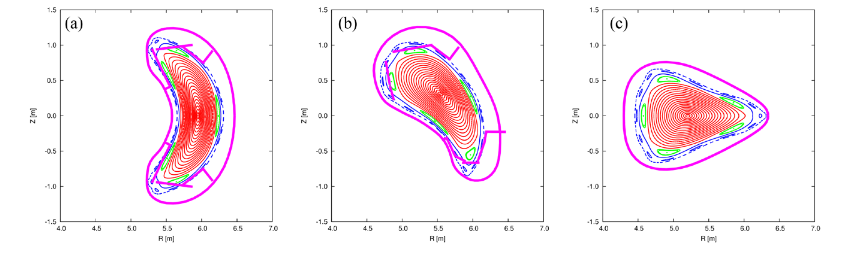
\includegraphics[scale = 0.8]{images/islands.png}
	\caption{Poincaré plots of the vacuum magnetic field in standard configuration for three different poloidal cross sections from \cite{Suzuki2016}. The islands intersecting the plasma facing components are shown in green, the target plates in pink.} \label{fig:1}
\end{figure}

The rotational transform can be varied between edge $\iota$ = 5/6 in the so-called low-iota configuration and edge $\iota$ = 4/5 in the high-iota configuration, with six and four magnetic islands respectively \cite{Knieps2021}. Following the island divertor concept \cite{Konig2002}, \cite{Renner2002}, target plates made of graphite intersect the islands to divert the heat and particle load and are shown in figure \ref{fig:1}.


\subsection{Heat load on the plasma facing components}

The heat load on the plasma facing components that intersect the islands is limited by the material properties of the plasma facing components and therefore needs to be monitored closely. While the divertor targets are designed for a heat flux of up to 10\,MW/m$^2$, significantly lower heat loads of 0.5\,MW/m$^2$ can be tolerated on the surrounding baffle structures \cite{Jakubowski2018}. Therefore, the surface temperature of the divertor targets and the surrounding structures are monitored closely by a set of infrared diagnostics to avoid overloading of the components and to study the particle and heat load deposition pattern on the plasma facing components. Based on the tenperature of the components, the heat flux can be derived using the two-dimensional thermal model THEODOR \cite{Sieglin2015}.
\begin{figure}[!htb]
	\centering
	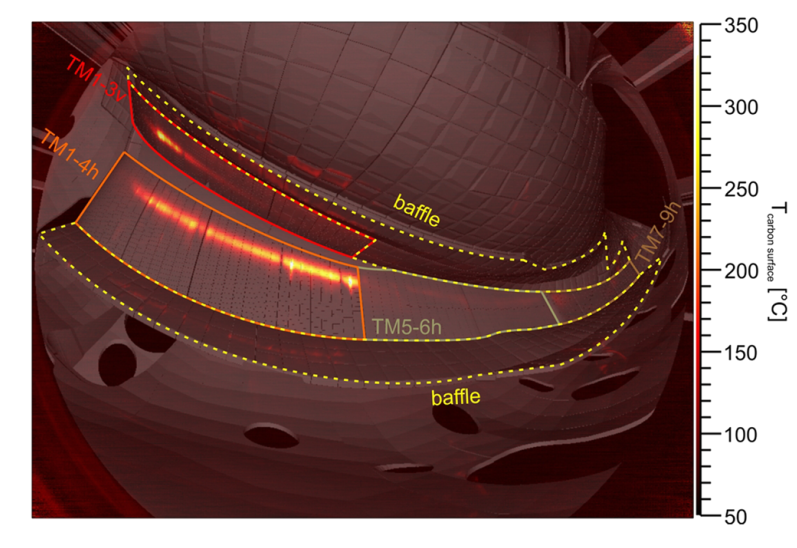
\includegraphics[scale = 0.5]{images/ir_image.png}
	\caption{Infrared image of one divertor module and the surrounding plasma facing components overlaid with a CAD model, from \cite{Jakubowski2018}} \label{fig:2}
\end{figure}
During the last experimental campaign, nine out of the ten divertor modules in Wendelstein 7-X - a lower and an upper divertor unit in each of the five modules of the torus - have been monitored by a set of different infrared and visible cameras. Infrared microbolometric cameras, which have been specifically designed to work in a magnetic field of up to 3\,T use a fish eye lens to provide a wide angle view of the whole divertor units. Detailed specifications of the cameras in use are given in \cite{Jakubowski2018}. The cameras provide a spectral response in the range of 8-10\,$\mu$m and can therefore be used to measure surface temperatures between 30 and 5000$^\circ$C. An example for the temperature distribution measured in one divertor unit is given in figure \ref{fig:2}, where the temperature distribution is overlaid by a CAD-model of the plasma facing components. This representation allows for a detailed sudy of the heat load deposition pattern on the plasma facing components \cite{Niemann2020} as well as the localization of individual thermal hotspots depending on the magnetic field configuration and the location of the magnetic islands. 









% INCLUDE: related work
% !TEX root = ../my-thesis.tex
%
\chapter{Principles of magnetic confinement}
\label{sec:principles}

\section{Non-axisymmetric magnetic fields}
In a fusion device or plasma experiment, the motion of the particles and thus the deposition of particle and heat load on the plasma facing components is inextricably linked to the magnetic field topology. Therefore, a short overview over magnetic confinement based on \cite{Helander2014} will be given in this section.\\
For confinement of a plasma, a magnetic field is required, which is related to the plasma current \textbf{J} by Ampere's law
\begin{equation}
    \nabla \times \textbf{B} = \mu_0\textbf{J}.
\end{equation}
The magnetic force created by the plasma current balances the pressure force of the plasma and enables confinement. The amount of plasma current needed for confinement can be derived from the MHD equation of motion which results in
\begin{equation}
    \textbf{J} \times \textbf{B} = \nabla p \label{eq2}
\end{equation}
for the steady state case without flows. As a consequence, \textbf{J} and \textbf{B} lie in surfaces of constant pressure, i.e.
\begin{equation}
    \textbf{B}\cdot \nabla p =  \textbf{J}\cdot \nabla p = 0.
    \label{eq3}
\end{equation}
These surfaces have toroidal topology in a magnetically confined plasma.
Magnetic coordinates are used to describe these surfaces of constant pressure in a coordinate system where one coordinate is constant on these surfaces and the magnetic field lines are straight lines. Introducing the poloidal and toroidal angles $\vartheta$ and $\varphi$, a representation of the magnetic field as a composition of the toroidal and poloidal component is given by
\begin{equation}
    \textbf{B} = \nabla \psi \times \nabla \theta + \nabla \varphi \times \nabla \chi
\end{equation}
with $ \theta = \vartheta + \lambda$.\\
According to \ref{eq3}, $\psi$ and $\chi$ are constant on surfaces of constant pressure and can be chosen to vanish on the innermost surface of constant pressure, that is just a line and described as the magnetic axis. By calculating the surface integral, it can be easily shown that the magnetic flux through a poloidal cross section of constant $\varphi$ between the magnetic axis and a surface of constant $\psi$ is equal to $2\pi\psi$, while the poloidal magnetic flux through a surface of constant $\phi$ between the magnetic axis and a flux surface $\psi$ is equal to $2\pi\chi$. These surfaces of constant toroidal and poloidal flux are called flux surfaces. \\
$\chi$ can be interpreted as the derivative of $\psi$, which is called the rotational transform
\begin{equation}
    \iota = \frac{d\chi}{d\psi}
\end{equation}
and indicates the number of poloidal turns per toroidal turn of a field line, because $\theta$ and $\varphi$ vary in proportion along a field line:
\begin{equation}
    \frac{d\phi}{d\varphi} = \frac{\textbf{B}\cdot \nabla \phi}{\textbf{B}\cdot \nabla \varphi} = \frac{(\nabla \varphi \times \nabla \chi) \cdot \nabla \phi}{(\nabla \psi \times \nabla \theta) \cdot \nabla \varphi} = \iota
\end{equation}
Introducing $\alpha = \theta - \iota \varphi$ leads to the so called Clebsch representation of the magnetic field
\begin{equation}
    \textbf{B} = \nabla \psi \times \nabla \alpha,
\end{equation}
where $\textbf{B} \cdot \nabla \alpha = 0$ and $\alpha$ is constant along the magnetic field. Consequently, the magnetic field lines are straight in the $(\theta, \varphi)$-plane, which was one of the requirements for the magnetic coordinates. Thus, the magnetic field lines can be described by the two coordinates $\psi$ and $\alpha$. Because $\frac{d\theta}{d\varphi} = \iota$ along a field line , the poloidal angle of a field line changes by $2\pi \iota$ after one toroidal turn. If $\iota$ is a rational number, i.e. $\iota = \frac{n}{m}$, the field line returns to where it started, while it traces out the whole flux surface for irrational $\iota$. \\

Although the magnetic field in stellarators is mainly generated by the magnetic field coils, the plasma current \textbf{J} that is needed to balance the plasma pressure modifies the magnetic field and consists of parallel and perpendicular components
\begin{equation}
    \textbf{J} = \textbf{J}_{\parallel} + \textbf{J}_{\perp}.
\end{equation}
The perpendicular component is required to produce the magnetic force given in \ref{eq2} and the parallel component is needed to satisfy \ref{eq3}. Thus, the current is given by
\begin{equation}
    \textbf{J} = (u(\psi, \theta, \varphi)p'(\psi)+\frac{\langle \textbf{J}_{\parallel}\textbf{B}\rangle}{\langle \textbf{B}^2\rangle}) \textbf{B}+\frac{\textbf{B} \times \nabla p}{B^2}, \label{eq9}
\end{equation}
where $u(\psi, \theta, \varphi)$ satisfies the magnetic differential equation $\textbf{B}\cdot \nabla u = -(\textbf{B}\times \nabla \psi) \cdot \nabla (\frac{1}{B^2})$. The first and second term in \ref{eq9} describe the parallel current, where the first one is the so-called Pfirsch-Schlüter current and the second term the Ohmic current. The third term describes the perpendicular diamagnetic current. A more detailed derivation of the plasma currents is given in \cite{Chen2012}. \\
While the existence of MHD equilibria \cite{Moffatt1985} can be proven e.g. using the variational principle \cite{Helander2014}, the pressure profiles or field lines do not necessarily have to be continuous or the plasma current free from singularities. A Fourier expansion of the parallel current in equation \ref{eq9} reveals the possible singularities in the current on the rational surfaces, namely a surface current and a divergent Pfirsch-Schlüter current. While a detailed derivation of these singularities can be found in \cite{Helander2014}, we do not focus on the discussion of singularities in the current here as they can be avoided by giving up on the requirement of nested flux surfaces and allowing for magnetic islands at rational surfaces. \\
The representation used for the magnetic field here,
\begin{equation}
    \textbf{B} = \nabla \times \textbf{A} = \nabla \psi \times \nabla \theta + \nabla \varphi \times \nabla \chi, \label{eq10}
\end{equation}
is a general repsresentation of the magnetic field and does not necessarily require the existance of magnetic surfaces.  They exist if $\chi$ can be written as a representation of $\psi$, since then $\textbf{B} \cdot \nabla \psi = 0$, but are not generally required. According to equation \ref{eq10}, the field lines are Hamiltonian
\begin{equation}
    \frac{d\psi}{d\varphi} = \frac{\textbf{B} \cdot \nabla \psi}{\textbf{B} \cdot \nabla \varphi} = - \frac{\partial \chi}{\partial \theta}
\end{equation}
\begin{equation}
    \frac{d\theta}{d\varphi} = \frac{\textbf{B} \cdot \nabla \theta}{\textbf{B} \cdot \nabla \varphi} =  \frac{\partial \chi}{\partial \psi}
\end{equation}
and are generally chaotic. The Hamiltonian $\chi$ can be Fourier decomposed, leading to
\begin{equation}
    \chi (\psi, \theta, \varphi) = \chi_0 (\psi) + \sum_{m, n\neq 0} \chi_{m,n}(\psi)e^{i(m\theta-n\varphi)} := \chi_0 (\psi) + f(\psi, \theta, \varphi).
\end{equation}
If $\psi$ and $\alpha = \theta-\iota(\psi_0)\varphi$ are used as canonical coordinates, , the Hamiltonian can be replaced by
\begin{equation}
    H(\psi, \alpha, \varphi) = \chi(\psi, \theta, \varphi)-\iota(\psi_0)(\psi-\psi_0) = \chi_0(\psi) + f(\psi, \alpha) - \iota(\psi_0)(\psi-\psi_0),
\end{equation}
which is equal to
\begin{equation}
    H(\psi, \alpha, \varphi) = \frac{\chi_0''(\psi_0)(\psi- \psi_0)^2}{2}+f(\psi_0, \alpha).
\end{equation}
This Hamiltonian can be integrated and described the magnetic islands around the resonant surface. The shape of the islands depends on the potential $f(\psi_0, \alpha)$. if only the first term is kept in the Fourier expansion, the potential becomes sinusoidal and the system is equivalent to an ordinary pendulum with the island separatrix corresponding to $2\chi_{mn}$ and
\begin{equation}
    \psi-\psi_0 = \sqrt{\frac{4\chi_{mn}(1-cos(m\alpha))}{\iota'(\psi_0)}}.
\end{equation}
The width of the islands is
\begin{equation}
    \Delta \psi = \sqrt{\frac{32\chi_{mn}}{\iota'(\psi_0)}}.
\end{equation}
As magnetic fields without continous symmetry are in general chaotic, they do not have nested flux surfaces everywhere and chains of islands can form, which consist if nested flux surfaces on their own with their own rotational transform. \\
The existence and calculation of such nested flux surfaces is carried out by the VMEC code based on the variational principle \cite{Hirshman1983},\cite{Hirshman1986}.

\section{Magnetic field in Wendelstein 7-X}
In the stellarator experiment Wendelstein 7-X \cite{Beidler1990},\cite{Klinger2013}, the magnetic field has been optimized for good MHD-stability and good neoclassical confinement \cite{Grieger1992}. It is the first device of the HELIAS line \cite{Nuhrenberg1986}, in which the plasma currents, i.e. the bootstrap current, the Pfirsch-Schlüter current and the diamagnetic current and their effects on the magnetic field are minimized \cite{Dinklage2018}.\\
The main magnetic field in Wendelstein 7-X is generated by 50 non-planar and 20 planar superconducting magnetic field coils that are cooled with liquid helium \cite{Rummel2012}. According to the five-fold symmetry of Wendelstein 7-X, there exist five different types of non-planar and two types of planar magnetic field coils made of NbTi, which are installed in each of the ten half modules of the stellarator. The flip-symmetric installation of two half modules results in the five identical modules composing Wendelstein 7-X. \\
The magnetic field generated by the coils and plasma currents determines the heat and particle load onto the plasma facing components, which are controlled by a chain of magnetic islands at the edge of the plasma. The number of islands depends on the edge rotational transform and is shown in figure \ref{fig:1} for the standard configuration, where an edge $\iota$ of 5/5 creates five islands.
\begin{figure}[!htb]
    \centering
    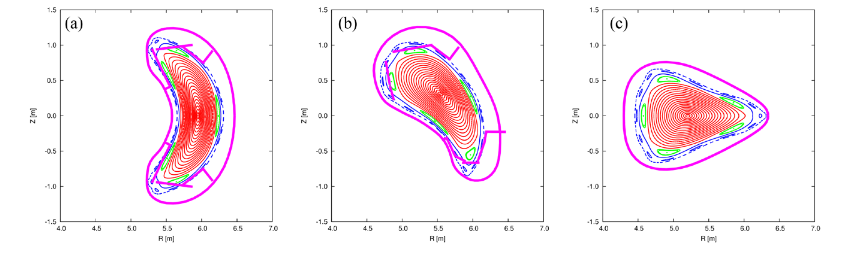
\includegraphics[width=\textwidth]{images/islands.png}
    \caption{Poincaré plots of the vacuum magnetic field in standard configuration for three different poloidal cross sections from \cite{Suzuki2016}. The islands intersecting the plasma facing components are shown in green, the target plates in pink.} \label{fig:1}
\end{figure}

The rotational transform can be varied between edge $\iota$ = 5/6 in the so-called low-iota configuration and edge $\iota$ = 4/5 in the high-iota configuration, with six and four magnetic islands respectively \cite{Knieps2021}. Following the island divertor concept \cite{Konig2002}, \cite{Renner2002}, target plates made of graphite intersect the islands to divert the heat and particle load and are shown in figure \ref{fig:1}.


\section{Heat load on the plasma facing components}

The heat load on the plasma facing components that intersect the islands is limited by the material properties of the plasma facing components and therefore needs to be monitored closely. While the divertor targets are designed for a heat flux of up to 10\,MW/m$^2$, significantly lower heat loads of 0.5\,MW/m$^2$ can be tolerated on the surrounding baffle structures \cite{Jakubowski2018}. Therefore, the surface temperature of the divertor targets and the surrounding structures are monitored closely by a set of infrared diagnostics to avoid overloading of the components and to study the particle and heat load deposition pattern on the plasma facing components. Based on the tenperature of the components, the heat flux can be derived using the two-dimensional thermal model THEODOR \cite{Sieglin2015}.
\begin{figure}[!htb]
    \centering
    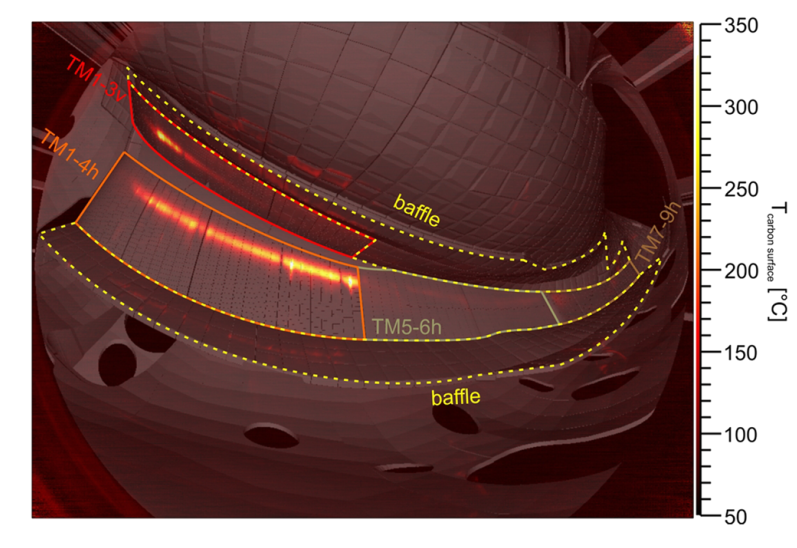
\includegraphics[scale = 0.5]{images/ir_image.png}
    \caption{Infrared image of one divertor module and the surrounding plasma facing components overlaid with a CAD model, from \cite{Jakubowski2018}} \label{fig:2}
\end{figure}
During the last experimental campaign, nine out of the ten divertor modules in Wendelstein 7-X - a lower and an upper divertor unit in each of the five modules of the torus - have been monitored by a set of different infrared and visible cameras. Infrared microbolometric cameras, which have been specifically designed to work in a magnetic field of up to 3\,T use a fish eye lens to provide a wide angle view of the whole divertor units. Detailed specifications of the cameras in use are given in \cite{Jakubowski2018}. The cameras provide a spectral response in the range of 8-10\,$\mu$m and can therefore be used to measure surface temperatures between 30 and 5000$^\circ$C. An example for the temperature distribution measured in one divertor unit is given in figure \ref{fig:2}, where the temperature distribution is overlaid by a CAD-model of the plasma facing components. This representation allows for a detailed sudy of the heat load deposition pattern on the plasma facing components \cite{Niemann2020} as well as the localization of individual thermal hotspots depending on the magnetic field configuration and the location of the magnetic islands.

% ToDo: Add some details about the coil configuration here

\begin{figure}[!htb]
    \centering
    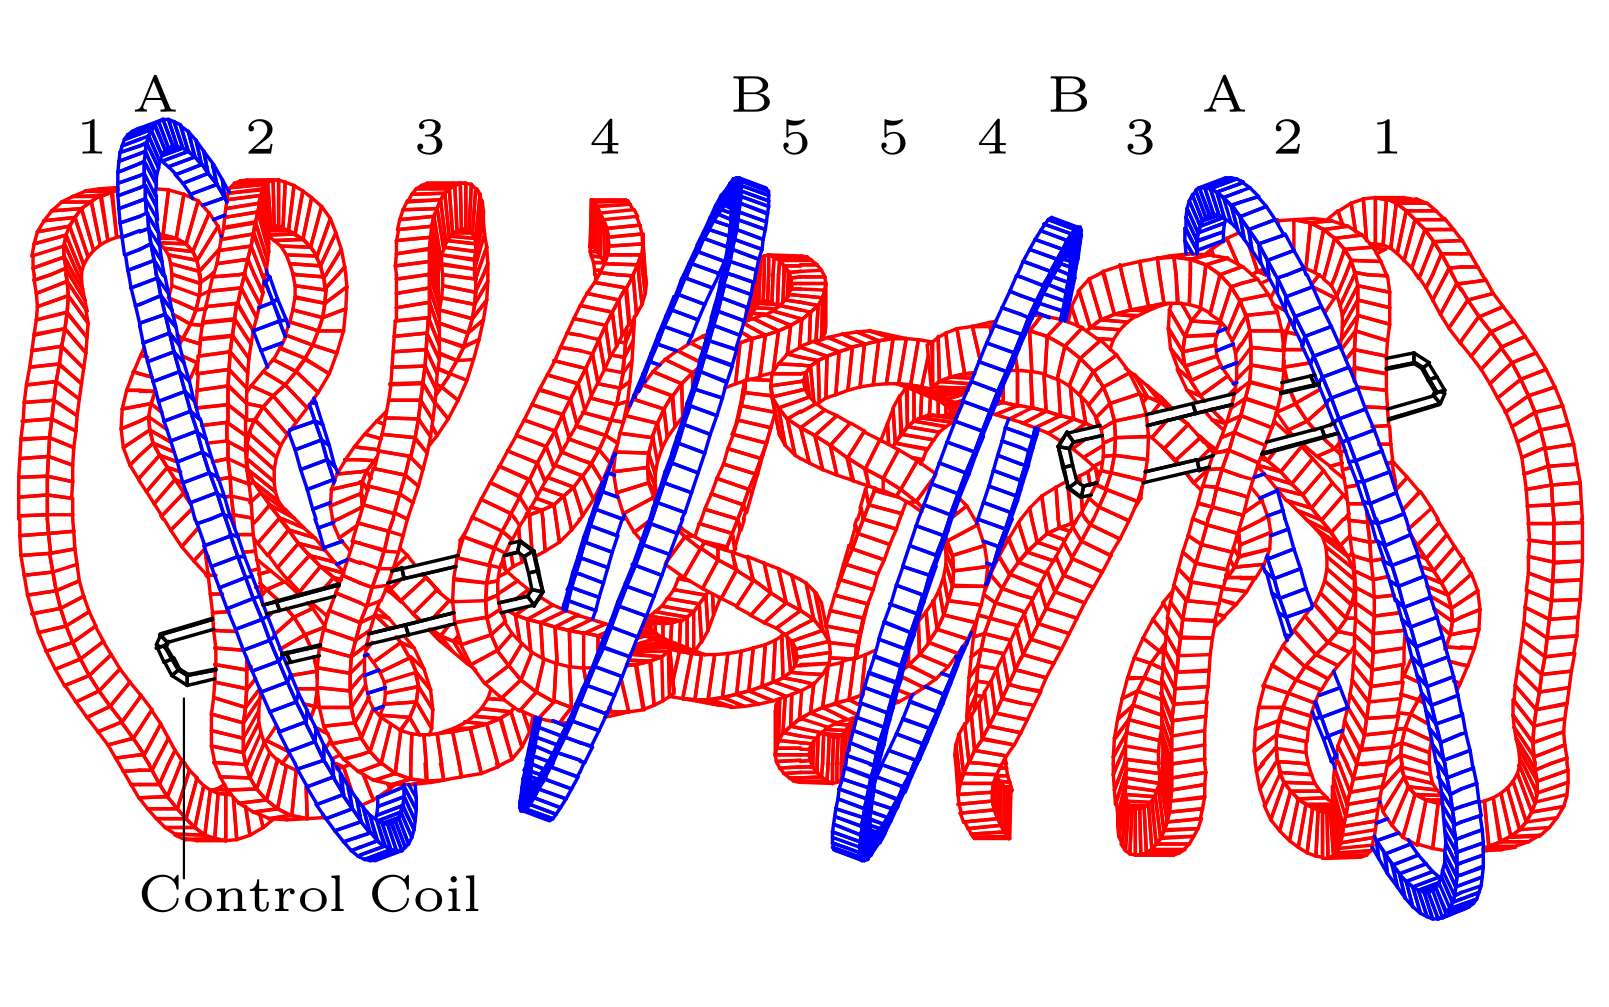
\includegraphics[scale = 0.7]{images/magnetic-coils.png}
    \caption{Coil diagram from one of the five W7X modules. The red coils are the non-planar coils. The blue coils are the two planar coils, $A$ and $B$. Taken from \ref{Böckenhoff_2018}} \label{fig:3}
\end{figure}
% INCLUDE: physics principles 
% !TEX root = ../my-thesis.tex
%
\chapter{Model Design}
\label{sec:code:model}

Machine learning (ML) models are algorithms that use data and statistical operations to optimize the weights that compose the model. There are two broad catagories of ML models, supervised and unsupervised. Supervised models are ones which use labeled data, or data for which the expected output of the model is known in advance. Unsupervised models are models for which a pattern is learned from the data directly. The model use for this project is a supervised ML model because we know what the expected inputs and outputs should be and can produce labels for both.

The primary input for the model will be thermal images taken from the infrared cameras at W-7X. Since the thermal camera data is sparse, with most of the pixels for any given shot containing zeros or noise, a convolutional neural network with that is optimized for sparse data would be ideal.

Convolutional neural networks use two dimensional convolutions applied to the inputs to generate new features (see Fig. \ref{fig:code:2DConv}). These convolutions are stacked, being applied to the same input to produce multiple outputs which are concatenated along the z-axis. Typically, strides (the number of pixels skipped over when translating the kernel) and padding (adding pixels around the edge of the image) allow convolutions to change the output x and y dimensions. So as more layers of convolutions are successively applied, the outputs of each layer grow in z-height, and shrink in x and y. The final output of the convolutional network is then passed to a fully connected network.


\begin{figure}[htb]
    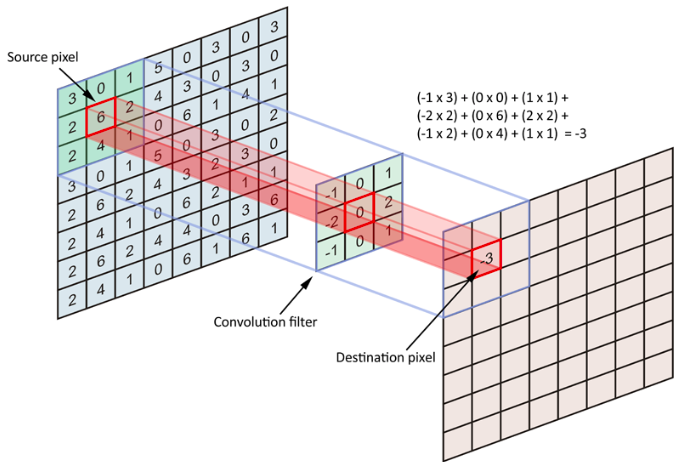
\includegraphics[width=\textwidth]{images/2d-Conv.png}
    \caption{Example of a single 3x3 convolution operation. The source image is convolved with a 3x3 kernel. The kernel's weights are determined using backpropagation. [cite source]}
    \label{fig:code:2DConv}
\end{figure}

\label{sec:code:inceptnet}

The inceptnet architecture [cite https://arxiv.org/abs/1409.4842] has been demonstrated by Böckenhoff [insert ref to Daniel's paper] to be effective on a simplified version of this problem. In initial tests it was was very promising for this application and met an important boundary conditions, mainly the network fit into the available video memory on the system used to train the network. Inceptnet uses a series of sub-networks, known as inception modules (see fig. \ref{fig:code:inceptmodule}). Each inception module is made up of 3 convolutional paths (1x1, 3x3, and 5x5) and a pooling path. To assure the outputs from each path have the same resolution, padding is added to the 3x3 and 5x5 convolutions. The number of each convolutional filter can be adjusted at each step and the outputs are concatenated together. The idea behind having multiple convolution sizes is that some features of the input might be lost if only size of kernel is applied.

\begin{figure}[htb]
    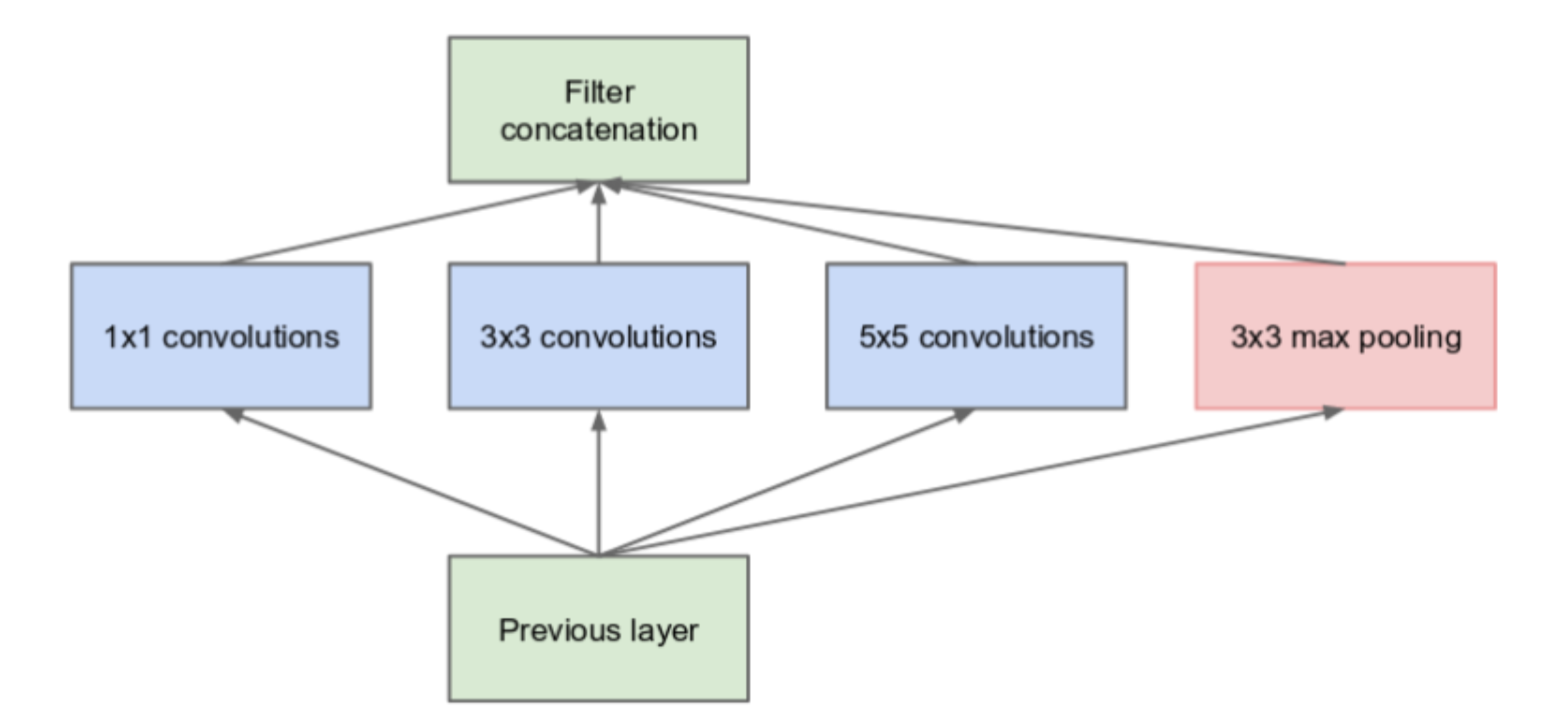
\includegraphics[width=\textwidth]{images/incept-simple.png}
    \caption{A diagram of the inception module. The inputs from the prior layer are fed into 4 paths, applying 1x1, 3x3, 5x5, convolutions with the final layer being 3x3 max pooling. The outputs of each layer are concatenated and passed to the next incept module. The number of 1x1, 3x3, and 5x5 convolutions per incept module can be adjusted.}
    \label{fig:code:inceptmodule}
\end{figure}

Each of the paths in the four branches of the inception module play a different role. The 1x1 filter doesn't take into account any patterns in the inputs height and width, but it does work across channels (depth) of the image. This acts to reduce the dimension of the input while connecting the values from the other channels of the input. Lin et. al in their 2014 paper [cite https://arxiv.org/pdf/1312.4400.pdf] referred to the 1x1 convolution as a "network in a network." The 1x1 convolution can also be used to reduce the number of channels as the output of the filter will be 1x1x$n$, where $n$ is the number of 1x1 filters being applied. This is why each branch has a 1x1 convolution. The 1x1 convolutions marked in yellow in fig. \ref{fig:code:inceptmodule} are designed to reduce the number of channels input to the higher computational cost which dramatically reduces the number of weights needed for a module.

The 3x3 and 5x5 convolutions look at spacial patterns across the width, height, and depth of the input. In this way they are actually a 3-dimensional convolution, but most convolutions are referred to by their 2 dimensional cross-section. These two filters are typical optimized for finding features of the input at different scales. Prior to this multi-branch approach, machine learning scientists would hand select the ordering of the various convolution sizes to be applied in succession. By providing multiple paths and allowing the training process to determine which branches are necessary for a given step takes the human bias out of the training process.

There are several other structures that appear in the inception module. One being a 3x3 max pooling layer, which is like a 3x3 convolution, but instead of taking the element-wise product with the filter, it returns the max pixel value over the region of the feature map that overlaps with the filter. Pooling layers are a method of downsampling the input while attempting to preserve the most relevant pixels and are a staple of most deep convolutional networks. The concatenation layer just concatenates the outputs from the various branches together. Each branch has padding so that the height and width channels are aligned to make concatenation simple.

Lastly, there are batch normalization layers after every operation on each brach of the inception module. Batch normalization is powerful tool in any deep learning model. It has been show by S. Ioffe and C. Szegedy in their 2015 paper [cite https://arxiv.org/pdf/1502.03167.pdf] that batch normalization largest solves the issue of internal covariate shift, where layers in the network shift the input distribution to the next layer. Since the inputs of any layer in the network are affected by the weights of every prior layer, small changes in the distribution get amplified as they propagate throughout the network. To address this during training batches of data are normalized, transforming the neurons output using the first and second statistical moments (mean and standard deviation) across the batch. Two additional trainable parameters, $\gamma$ and $\beta$ are applied after normalization to specify the output distribution, so each layer can achieve a unique output distribution based on the optimal one for the next operation or layer.

Incept modules also have two major advantages over classic deep convolutional networks, they require far fewer parameters, which reduced the overall memory footprint of the model and far fewer floating point operations than prior convolutional modules. For example, using a 5x5 convolution to produce the same number of output channels as a incept module requires over 7 times the number of model parameters and floating point operations compared to the incept module. However, despite having significantly fewer model parameters, when the inceptnet was release, it was the state of the art architecture. Inceptnet outperformed models with the higher parameter count 5x5 and 3x3 modules.

The inception modules are stacked repeatedly (see fig. /ref{}), varying the number of filters in each brach of the incept modules in each layer of modules. Eight total inception modules were used in the network with an input and output network. The input network is a 2D convolution used to scale up the number of channels. The output network flattens the output and passes it though a 128 neuron fully connected layer before reducing it to the output dimension of the network. While this was a reduction in the original scale of the Inceptnet design because the input images are higher resolution there are far more weights per step. For example, with an image resolution of 80\% of the original image size (260x1040 pixels) and a batch size of 10, the amount of ram needed to store the weights for the forward and back propagation step alone is 21.4 GB, which exceeds the video memory of all but the highest end consumer graphics cards. Since one of the questions being addressed by this thesis will be the impact of scaling the input image resolution on the accuracy, it is important to design a model that can will run with the hardware available.

\label{sec:code:hyperparameters}

Once the broad architecture was selected the next step is to tune the model. Tuning the model helps model level parameters, like the number of filters at a given module, to be optimized for the use case. Tuning was done systematically with Optuna and results were recorded and compared using Tensorboard and MLFlow. You can see from the table [Insert graph] the results of tuning the hyperparameter for the optimization step size $\alpha$.

The labels of the data set are the expected values the network will output given a specific input.
$\iota$, the rotational transform or the ratio of poloidal transits per toroidal turn of any field line on a flux surface, is the label used for training. Initially, the labels for the data set were not available since simulations were necessary to produce them and that process takes a great deal of time.Instead, simplified versions of the labels which just took into account the sum of $I_A$ and $I_B$, which provides a good first order approximation [inset /ref{} to eq]. Naturally, this will neglect the plasmas induced changes to the magnetic field. Simulations using VMEC, a plasma physics simulation framework, allowed for a more accurate approximation for $\iota$. However, it is prohibitively computationally intensive to run 22,000+ simulations using the field line tracer, a simulation tool necessary for extending the results from VMEC to regions outside of the plasma. The compromise is use a value if $\iota$ at the edge of the plasma, as the VMEC simulations can be made much faster alone.

\label{sec:code:philosophy}
The design philosophy of this project was important. The code was designed to be a complete package, to be easily used by fellow colleges, and to work with the state of the art tools available in the machine learning space. PyTorch was used at the primary framework, as many of members of the NEISS group used this as well. The PyTorch Lightning package provided a powerful way to design an object-oriented machine learning package. For lower-level operations, like managing and recording the network configuration files, hyperparmeter searches, as well as structuring and analyzing results, the package Hydra, developed by Facebook, was used. Git was used for the version control system and DVC for data version control. This project was profiled and optimized with help from the PyTorch Lightning profiler. Code comments and documentation have been developed to help with quick adoption of the code for future use.

Since future changes to the divertor surface will result in drastically different inputs to the network, the code was designed to automatically scale with the inputs. The design philosophy was focused on making a project that could be quickly and easily taken over by a future student and be powerful and flexible enough to work with expected changes in the future. Even if the code is never used again it was still a valuable lesson in Python software development.



% \section{Postcards: My Address}
% \label{sec:intro:address}

% \textbf{Ricardo Langner} \\
% Alfred-Schrapel-Str. 7 \\
% 01307 Dresden \\
% Germany



% \section{Motivation and Problem Statement}
% \label{sec:intro:motivation}

% \Blindtext[3][1] \cite{Jurgens:2000,Jurgens:1995,Miede:2011,Kohm:2011,Apple:keynote:2010,Apple:numbers:2010,Apple:pages:2010}

% \section{Results}
% \label{sec:intro:results}

% \Blindtext[1][2]

% \subsection{Some References}
% \label{sec:intro:results:refs}

% \cite{WEB:GNU:GPL:2010,WEB:Miede:2011}
% \Blindtext[1][1]

% \subsubsection{Methodology}
% \label{sec:intro:results:refs:method}

% \Blindtext[1][2]

% \paragraph{Strategy 1}
% \Blindtext[1][1]

% \begin{lstlisting}[language=Python, caption={This simple helloworld.py file prints Hello World.}\label{lst:pyhelloworld}]
% #!/usr/bin/env python
% print "Hello World"
% \end{lstlisting}

% \paragraph{Strategy 2}
% \Blindtext[1][1]

% \begin{lstlisting}[language=Python, caption={This is a bubble sort function.}\label{lst:pybubblesort}]
% #!/usr/bin/env python
% def bubble_sort(list):
%     for num in range(len(list)-1,0,-1):
%         for i in range(num):
%             if list[i]>list[i+1]:
%                 tmp = list[i]
%                 list[i] = list[i+1]
%                 list[i+1] = tmp

% alist = [34,67,2,4,65,16,17,95,20,31]
% bubble_sort(list)
% print(list)
% \end{lstlisting}

% \section{Thesis Structure}
% \label{sec:intro:structure}

% \textbf{Chapter \ref{sec:related}} \\[0.2em]
% \blindtext

% \textbf{Chapter \ref{sec:system}} \\[0.2em]
% \blindtext

% \textbf{Chapter \ref{sec:concepts}} \\[0.2em]
% \blindtext

% \textbf{Chapter \ref{sec:concepts}} \\[0.2em]
% \blindtext

% \textbf{Chapter \ref{sec:conclusion}} \\[0.2em]
% \blindtext
    % INCLUDE: code design
%\part{Additional Example Part}
% !TEX root = ../my-thesis.tex
%
\chapter{System}
\label{sec:system}

\cleanchapterquote{Innovation distinguishes between a leader and a follower.}{Steve Jobs}{(CEO Apple Inc.)}

\Blindtext[2][1]

\section{System Section 1}
\label{sec:system:sec1}

\Blindtext[1][2]

\begin{figure}[htb]
	
\includegraphics[width=\textwidth]{gfx/Clean-Thesis-Figure}
	\caption{Figure example: \textit{(a)} example part one, \textit{(c)} example part two; \textit{(c)} example part three}
	\label{fig:system:example1}
\end{figure}

\Blindtext[1][2]

\section{System Section 2}
\label{sec:system:sec2}

\Blindtext[1][2]

\begin{figure}[htb]
	
\includegraphics[width=\textwidth]{gfx/Clean-Thesis-Figure}
	\caption{Another Figure example: \textit{(a)} example part one, \textit{(c)} example part two; \textit{(c)} example part three}
	\label{fig:system:example2}
\end{figure}

\Blindtext[2][2]

\section{System Section 3}
\label{sec:system:sec3}

\Blindtext[4][2]

\section{Conclusion}
\label{sec:system:conclusion}

\Blindtext[2][1]
         % INCLUDE: system
% !TEX root = ../my-thesis.tex
%
\chapter{Concepts: This text is here to test a very long title, to simulate the line break behavior, to show that an extremely long title also works}
\label{sec:concepts}

\cleanchapterquote{Users do not care about what is inside the box, as long as the box does what they need done.}{Jef Raskin}{about Human Computer Interfaces}

\Blindtext[2][1]

\section{Concepts Section 1}
\label{sec:concepts:sec1}

\Blindtext[2][2]

\section{Concepts Section 2 with a very very long title that illustrates how long section titles are handled in the footer}
\label{sec:concepts:sec2}

\Blindtext[3][2]

\section{Concepts Section 3}
\label{sec:concepts:sec3}

\Blindtext[4][2]

\section{Conclusion}
\label{sec:concepts:conclusion}

\Blindtext[2][1]

% !TEX root = ../my-thesis.tex
%
\chapter{Results}
\label{sec:results}

\section{Input resolution scaling}

Better understanding the impact of input resolution on the neural network training results is important for optimizing the network. The neural network was trained on inputs of varying resolution. The resolution of the inputs was scaled and the network parameters were scaled according to the inputs, so larger resolution images also had more network parameters.

In table \ref{table:input} the input resolutions and the corresponding number of multiply–accumulate operations (MAC) are presented. MACs are a commonly used metric in machine learning because many of the tensor optimized accelerators compute $a \cdot x+b$ as a single operation \cite{nvidia_technical_blog_2022}, therefore one MAC is approximately 2 floating point operations (FLOPS).

\begin{table}
    \begin{tabular}{ |p{3cm}|p{3cm}|p{4cm}|  }
        \hline
        \multicolumn{3}{|c|}{Network input resolution, number of multiply–accumulate operations.} \\
        \hline
        x resolution & y resolution & MAC (G)                                                     \\
        \hline
        780          & 195          & 235.15                                                      \\
        520          & 130          & 104.39                                                      \\
        260          & 65           & 26.31                                                       \\
        156          & 39           & 9.49                                                        \\
        104          & 26           & 5.65                                                        \\
        52           & 13           & 1.09                                                        \\
        \hline
    \end{tabular}
    \caption{Input resolutions for six neural network architectures and corresponding multiply–accumulate operations as a measure of the computational resources needed to train the network. To facilitate the larger input size the network adjusts the number of parameters, which results in an increase of computational resources to train.}
    \label{table:input}
\end{table}

When scaling the resolution to the labels used by the neural network, it can been seen in figure \ref{fig:resolution-scaling} that higher resolution inputs do not necessarily result in better training results. In the case of the inception network that was tested, larger input resolutions also result in higher numbers of parameters and longer training times. The larger number of parameters could make it easier to overfit the network, especially with the limited size of the data set. However, when the resolution of the inputs is below 16900 pixels (260x65), the network is unable to resolve the features necessary to achieve an $rmse$ below $6 \cdot 10^{-3}$. If more training data was available, the network would be able to learn the features necessary to achieve a lower $rmse$ at the same resolution.

\begin{figure}[!htb]
    \centering
    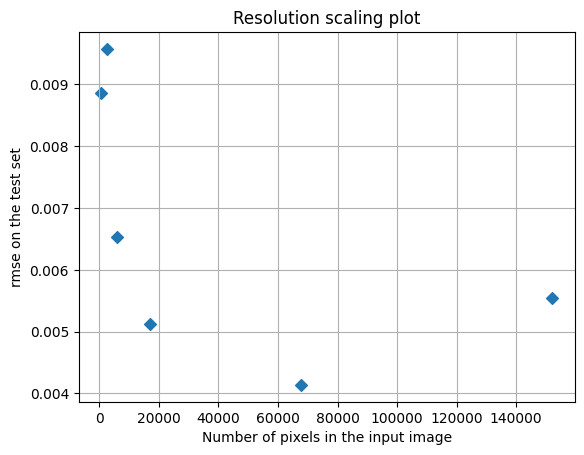
\includegraphics[width = \textwidth]{images/resolution-scaling.png}
    \caption{$rmse$ after training the neural network on the inputs at a given resolution over number of pixels in the input image. The pixel values are a product of the input image from the thermal camera height and width values after being scaled.} \label{fig:resolution-scaling}
\end{figure}

\section{Network Performance}

It is difficult to completely disentangle the increased network performance from the increased number of network parameters. However, it is not necessary to do so because ultimately the goal is to find a network that can be trained in a reasonable amount of time and that can be used to predict $\bar{\iota}$ values. The increased computational cost of training the network amounts to a few hours of training time on a single GPU. The network that was trained on the 520x130 input images was able to achieve this goal. The 520x130 network was able to achieve an $rmse$ of $4.13 \cdot 10^{-3}$ in 8 hours of training time on a single GPU, and the next best result was given by the 260x65 network with an $rmse$ of $5.12 \cdot 10^{-3}$ for a 50\% reduction in overall training time.

Figure \ref{fig:iota_vs_pred} shows the simulated $\bar{\iota}$ values vs the neural network reconstruction of $\bar{\iota}$ for the validation and test data sets for the two highest performance networks. As mentioned in section \ref{sec:data}, the neural network was trained on a data set that was split into training, validation, and test data sets but the distribution of $\bar{\iota}$ values was not uniform. This can be clearly seen in this graph, with the five independent programs worth of data being used for testing. The values for the test data set are normalized to mean zero and standard deviation one for the purposes of this plot, but in the actual training the training data set was used to normalize the test data. The reconstructed $\bar\iota$ values are then normalized to the test set. It can be seen in the right plot, the network slightly overestimates lower $\bar{\iota}$ values and slightly underestimates higher $\bar{\iota}$ values. The left plot, which shows the highest performance model does not show as much bias as the right plot, but the bias is still present. The bias is likely due to the limited size of the data set and the limited distribution of $\bar{\iota}$ values.


\begin{figure}[!htb]
    \centering
    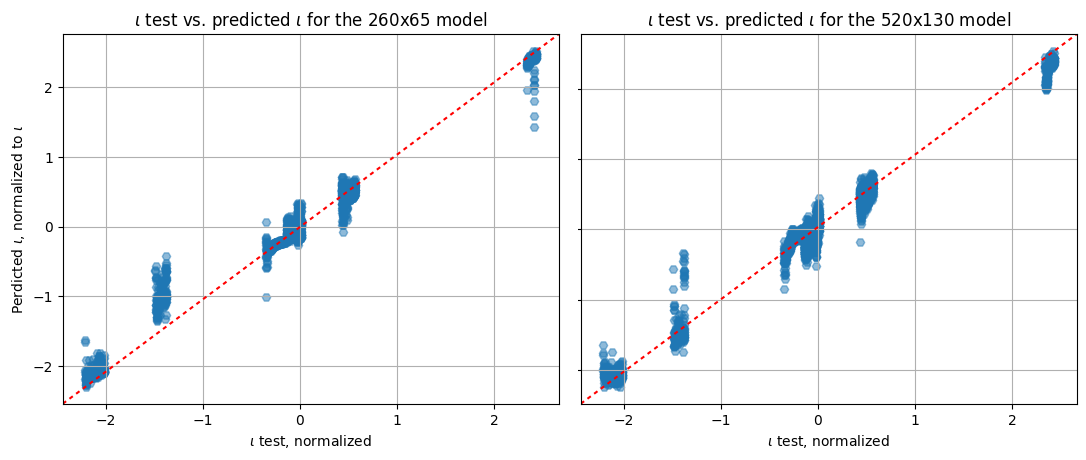
\includegraphics[width = \textwidth]{images/iota_vs_pred.png}
    \caption{$\bar{\iota}$ reconstruction with top two networks.} \label{fig:iota_vs_pred}
\end{figure}

A similar trend can be seen in the violin plots in figure \ref{fig:kde}. In this plot the distribution of the L2 error kernel density estimate (KDE) is shown for all six networks. It should be noted that the KDE is not a probability distribution, but it is a good way to visualize the distribution of the error, and it is a good way to compare the error distributions of the different networks. The point-wise L2 error is defined as:

\begin{equation}
    \label{eq:l2}
    \text{L2 error} = (y_i - \hat{y}_i)^2
\end{equation}

where $y_i$ is the true value of $\bar{\iota}$ and $\hat{y}_i$ is the predicted value of $\bar{\iota}$. KDE is defined as:

\begin{equation}
    \label{eq:kde}
    \text{KDE} = \frac{1}{n} \sum_{i=1}^n \frac{1}{h} \sum_{j=1}^n K\left(\frac{y_i - y_j}{h}\right)
\end{equation}

where $n$ is the number of data points, $h$ is the bandwidth of the kernel, and $K$ is the kernel function. The bandwidth is chosen to be $0.1$ for all of the KDE plots. The kernel function used is the Gaussian kernel:

\begin{equation}
    \label{eq:gaussian}
    K(x) = \frac{1}{\sqrt{2 \pi}} e^{-\frac{x^2}{2}}
\end{equation}

Since values below zero are irrelevant to L2 error, the distributions are truncated at zero. The KDE is calculated for each network and then the KDE is normalized to the entire dataset. The KDE is then plotted as a violin plot, which is a box plot with the kernel density estimate plotted as a density function. The KDE is plotted as a density function because it is not a probability distribution. The two networks that exhibit best performance can be seen to have higher q-factors than the other networks.

\begin{figure}[!htb]
    \centering
    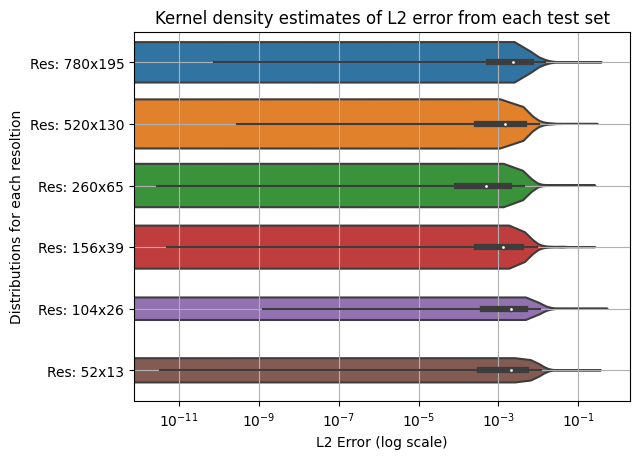
\includegraphics[width = \textwidth]{images/kde_plot.png}
    \caption{Kernel density estimate of L2 error from each trained neural network on the test datasets.} \label{fig:kde}
\end{figure}

       % INCLUDE: concepts
% !TEX root = ../my-thesis.tex
%
\chapter{Conclusion}
\label{sec:conclusion}

In conclusion, this thesis presents a successful approach for inferring the edge rotational transform, $\bar{\iota}$, of the Wendelstein 7-X plasma experiment from heat load data. By training an inceptnet convolutional neural network on a dataset of infrared camera images, the network was able to infer the edge rotational transform with an $rmse$ of $4.13 \cdot 10^{-3}$. This is an improvement over prior work with similar data and indicates that the proposed approach is a viable solution for determining real-time extraction of $\bar{\iota}$ from the W7-X experiment. Since the network was trained on inputs with a 520x130 resolution, which is a good compromise between computational cost and network performance, further improvements . The training time for the network was less than a day on a single GPU, making it a practical solution for use in the W7-X. Overall, this work demonstrates the potential of using machine learning techniques to improve the control and performance of plasma experiments such as the W7-X.     % INCLUDE: conclusion

% --------------------------
% Back matter
% --------------------------
%
{%
    \setstretch{1.1}
    \renewcommand{\bibfont}{\normalfont\small}
    \setlength{\biblabelsep}{0pt}
    \setlength{\bibitemsep}{0.5\baselineskip plus 0.5\baselineskip}
    \printbibliography[nottype=online]
    \newrefcontext[labelprefix={@}]
    \printbibliography[heading=subbibliography,title={Webpages},type=online]
}
\cleardoublepage

\listoffigures
\cleardoublepage

\listoftables
\cleardoublepage

\lstlistoflistings
\cleardoublepage

\appendix\cleardoublepage
% !TEX root = ../my-thesis.tex
%
\chapter{Example Appendix}
\label{sec:appendix}

\Blindtext[1][1]

\section{Appendix Section 1}
\label{sec:appendix:sec1}

\Blindtext[1][1]

\begin{table}[h]
	\begin{tabularx}{\textwidth}{X | X | X}
		%\hline
		Alpha		& Beta			& Gamma			\\ \hline
		0			& 1				& 2				\\ \hline
		3			& 4				& 5				\\ %\hline
	\end{tabularx}
	\label{tab:table1}
	\caption{This is a caption text.}
\end{table}

\section{Appendix Section 2}
\label{sec:appendix:sec2}

\Blindtext[1][1]

\begin{table}[h]
	\begin{tabularx}{\textwidth}{X | X | X}
		%\hline
		Alpha		& Beta			& Gamma			\\ \hline
		0			& 1				& 2				\\ \hline
		3			& 4				& 5				\\ %\hline
	\end{tabularx}
	\label{tab:table2}
	\caption{This is a caption text.}
\end{table}

\Blindtext[1][2]
       % INCLUDE: appendix

\cleardoublepage
% !TEX root = ../my-thesis.tex
%
\pagestyle{empty}
\hfill
\vfill
\pdfbookmark[0]{Colophon}{Colophon}
\section*{Colophon}

This thesis was typeset with \LaTeXe.
It uses the \textit{Clean Thesis} style developed by Ricardo Langner.
The design of the \textit{Clean Thesis} style is inspired by user guide documents from Apple Inc.

Download the \textit{Clean Thesis} style at \url{http://cleanthesis.der-ric.de/}.


\cleardoublepage
% !TEX root = ../my-thesis.tex
%
%************************************************
% Declaration
%************************************************
\pdfbookmark[0]{Declaration}{Declaration}
\addchap{Declaration}
\label{sec:declaration}
\thispagestyle{empty}

You can put your declaration here, to declare that you have completed your work solely and only with the help of the references you mentioned.

\bigskip

\noindent\textit{\thesisUniversityCity, \thesisDate}

\smallskip

\begin{flushright}
	\begin{minipage}{5cm}
		\rule{\textwidth}{1pt}
		\centering\thesisName
	\end{minipage}
\end{flushright}

%*****************************************
%*****************************************

\clearpage

\newpage
\mbox{}

% **************************************************
% End of Document CONTENT
% **************************************************
\end{document}
